\chapter{Method}

% \section{Voxelnet}
% VoxelNet is an End-to-End Learning for Point Cloud Based 3D Object Detection. The work is described in Yin Zhou and Oncel Tuzel's paper: \cite{https://doi.org/10.48550/arxiv.1711.06396}.

% In order to implement this work, the following git repo is adapted: \url{https://github.com/qianguih/voxelnet}. This repo contains a pre-trained model, trained to detect cars from the velodyne lidar data provided by the KITTI dataset.

% \section{ViperX 300 Robot Arm}
% In order to operate the Trossen Robotics ViperX 300 Robotic Arm, Their ROS 2 packages are utilised.
% These can be found here: \url{https://docs.trossenrobotics.com/interbotix_xsarms_docs/}.

This chapter will describe different methodologies used to solve technical problems over the course of this project.

\section{Problem Formulation}

The objective of this project is to set up an autonomous warehouse system where an autonomous UGV should be able to fetch objects in a warehouse. The system will rely on an UGV equipped for autonomous navigation to move around in the environment. The UGV will also be equipped with a robotic manipulator for pick and place operations.

\section{Conceptual Design}
The design of the robot should reflect the intended tasks of the robotic platform. For an autonomous warehouse robot, these tasks involve autonomous navigation, pick and place and object detection/recognition. The design should deliver a platform that could be used for future projects. 

\subsection{Initial Concept}
With the described design specifications considered, the initial conceptual design resulted in the following major components:

\begin{itemize}
    \item Clearpath - Husky A200 UGV
    \item Redshift Labs - UM7 IMU
    \item Ouster -  OS1-64 3D LiDAR
    \item Universal Robots - UR5
    \item Intel - Realsense D435i Camera
    \item 2 X NVIDIA - Jetson AGX Xavier
\end{itemize}

From the bulletin list above, Husky A200, seen in figure \ref{fig:huskyA200}, provides a robust mobile platform and UM7 IMU and Ouster OS1-64 LiDAR provides sensory information to allow for autonomous navigation. The UR5 robotic manipulator, seen in figure \ref{fig:ur5}, paired with an Intel Realsense D435i, adds capabilities for pick and place operations with object detection and 6-DOF pose estimation. The two NVIDIA Jetson AGX Xaviers will be used to control the platform.

\begin{figure}[H]
  \centering
  \begin{minipage}[b]{0.49\textwidth}
        \centering
        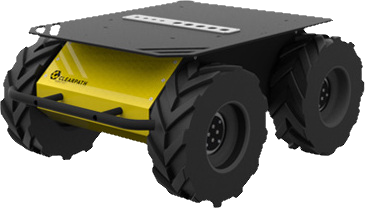
\includegraphics[width = 0.8\textwidth]{Figures/huskyA200.png}
        \caption{Clearpath Husky A200. Image adapted from \cite{clearpath_husky_website}}
        \label{fig:huskyA200}
  \end{minipage}
  \hfill
  \begin{minipage}[b]{0.49\textwidth}
    \centering
    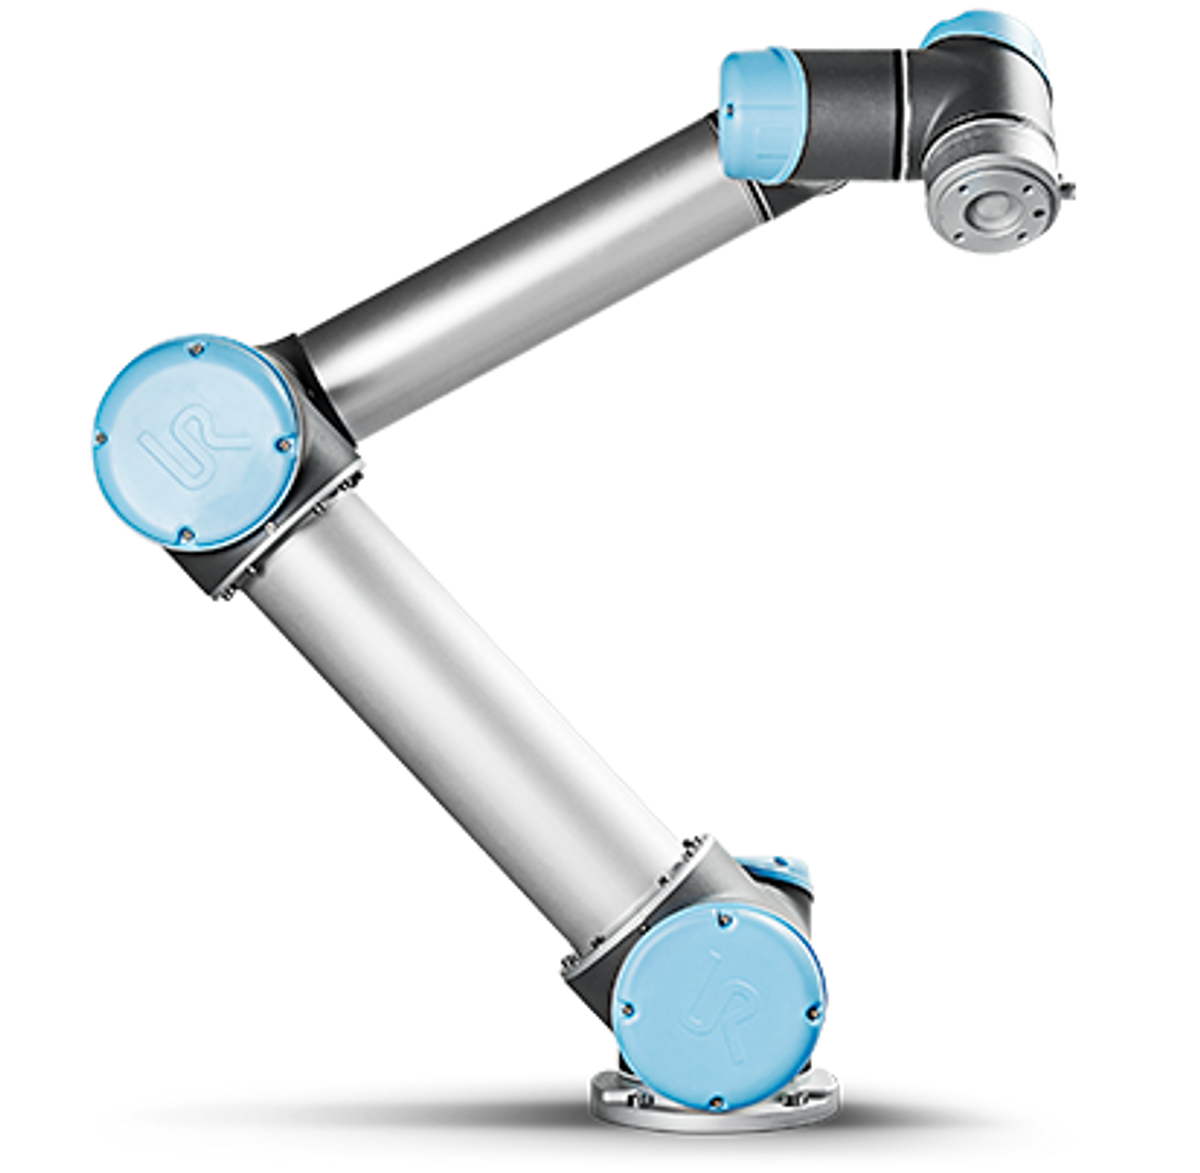
\includegraphics[width = 0.8\textwidth]{Figures/ur5.png}
    \caption{Universal Robots UR5. Image from \cite{ur5_img}}
    \label{fig:ur5}
  \end{minipage}
\end{figure}

Some specifications on the Husky A200 robotic platform is listed in table \ref{tab:husky:a200:specs}

\begin{table}[H]
\centering
\caption{Technical specifications for the Clearpath Husky A200, complete data sheet available in appendix \ref{A:fig:husky_data_sheet}, from \cite{clearpath_husky_website}}
\label{tab:husky:a200:specs}
\vspace{1mm}
\begin{tabular}{ll}
\hline
\multicolumn{2}{c}{\textbf{Husky A200 Specifications}}                                                            \\ \hline
Drivers and APIs                            & ROS, ROS 2, C++ and Python                                          \\
Wheel encoders                              & Quadrature: 78,000 {[}pulses/m{]}
        \\
Communication                               & RS232@115200 Baud                                                   \\
Battery                                     & \begin{tabular}[c]{@{}l@{}}12V 20Ah\\ Sealed Lead Acid\end{tabular} \\
\multicolumn{1}{c}{User Power Distribution} & \begin{tabular}[c]{@{}l@{}}5V 5A\\  12V 5A\\  24V 5A\end{tabular}   \\
Weight                                      & 50 {[}kg{]}                                                         \\
Payload Capacity                            & 75 {[}kg{]}                                                         \\
External Dimensions                         & 990 x 670 x 390 {[}mm{]}                                            \\ \hline
\end{tabular}
\end{table}

One NVIDIA Jetson AGX Xavier, hereby called "UGV Xavier", interfaces with Husky, LiDAR and IMU. This computer will control the Husky and take care of autonomous navigation tasks such as mapping, localization and path planning. 

The second NVIDIA Jetson AGX Xavier, hereby called Manipulator Xavier, interfaces with the Realsense camera and robotic manipulator. This computer will control the manipulator, and take care of sensory information from the Realsense camera. 

The relatively powerful GPU of the Xaviers adds capabilities to implement deep learning algorithms to do for example image- or PointCloud based object detection.

\subsection{Final Design/Concept??}
The final design is 

\subsection{Topology}
Looking at figure \ref{fig:topology}, it can be seen that the UGV Xavier communicates with the Husky through RS232 and the UM7 IMU through USB. The LiDAR communicates through Ethernet via a WiFi router that acts as a switch. It's data is therefore available for all computers on the network. From figure \ref{fig:topology}, it can be seen that the Manipulator Xavier interfaces with both the Realsense camera and the manipulator through USB.

\begin{figure}[H]
  \centering
  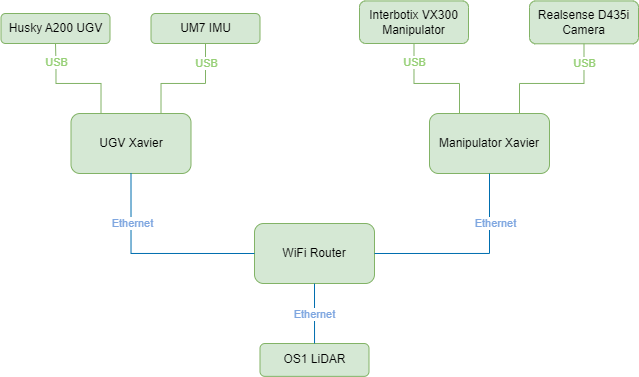
\includegraphics[width = 0.6\textwidth]{Figures/example_figure.drawio.png}
  \caption{High level topology of the mobile robotic platform}
  \label{fig:topology}
\end{figure}


  
\section{Hardware Setup}


The complete setup is described in URDF files, which allows for an accurate digital model of the robot to be made . The URDF model of the robot is shown in figure \ref{fig:hardware}.

\begin{figure}[H]
  \centering
  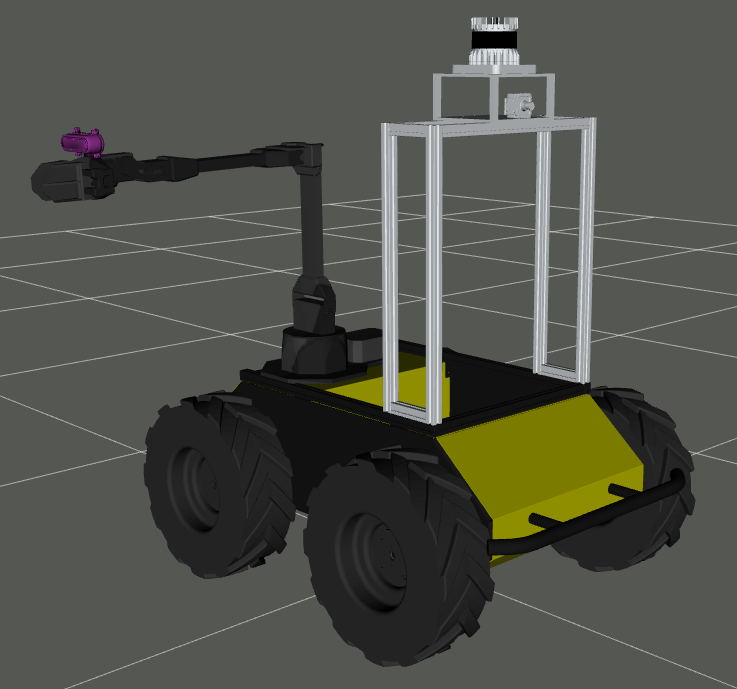
\includegraphics[width = 0.6\textwidth]{Figures/husky_initiated.png}
  \caption{3D model of the robotic system.}
  \label{fig:hardware}
\end{figure}


\section{Autonomous Navigation}
Autonomous navigation is achieved using the NAV2 navigation stack for ROS 2.

\section{Autonomous Object Fetching}
On a high level, the system is controlled by a ros node called "husky\_master". This node interacts with NAV2 and Moveit 2 to orchestrate an autonomous pick and place operation. The interaction between "husky\_master" and Moveit 2 is done through "husky\_pick\_and\_place" which acts as an interface between Moveit 2 and "husky\_master". A high level overview of this interaction is shown in figure \ref{fig:software_overview}

\begin{figure}[H]
  \centering
  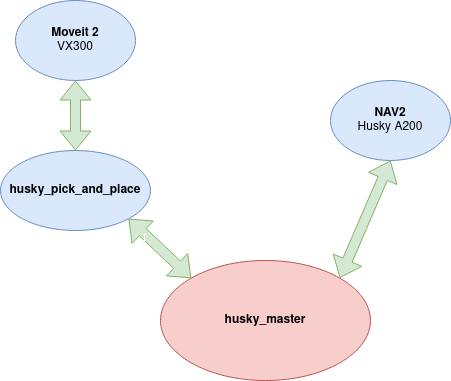
\includegraphics[width = 0.6\textwidth]{Figures/software_overview.drawio.png}
  \caption{Software overview of warehouse automation system. The "husky\_master" node controls the operation by interfacing directly with NAV2 and with Moveit2 trhough the "husky\_pick\_and\_place" node.}
  \label{fig:software_overview}
\end{figure}